\documentclass[titlepage,10pt,openany]{scrbook}
\usepackage[papersize={107.5mm,148.5mm},twoside,bindingoffset=0.5cm,hmargin={1cm,1cm},				vmargin={1.5cm,1.5cm},footskip=0.5cm,driver=dvipdfm]{geometry}

%\usepackage[papersize={148.5mm,215mm},twoside,bindingoffset=0.5cm,hmargin={1cm,1cm},				vmargin={1.5cm,1.5cm},footskip=0.5cm,driver=dvipdfm]{geometry}

\usepackage[T1]{fontenc}
\usepackage{lmodern}
\usepackage{url}
\usepackage[svgnames]{xcolor}
%\usepackage[utf8]{inputenc}
\usepackage{graphicx}
\usepackage{wrapfig}
\usepackage[bahasa]{babel}
\usepackage{fancyhdr}
\usepackage{pifont}
\usepackage{microtype}
\usepackage{pst-text}
\usepackage{palatino}
\usepackage{marvosym}
\usepackage{pdfpages}
\usepackage{hyphenat}
\usepackage{tikz}
\usepackage{pdfcolmk}


\makeatletter
%%%% light series
%% e.g., kernel doc, section s: line 12 or thereabouts
\DeclareRobustCommand\ltseries
{\not@math@alphabet\ltseries\relax
	\fontseries\ltdefault\selectfont}
%% e.g., kernel doc, section t: line 32 or thereabouts
\newcommand{\ltdefault}{l}
%% e.g., kernel doc, section v: line 19 or thereabouts

\DeclareTextFontCommand{\textlt}{\ltseries}
% heavy(bold) series
\DeclareRobustCommand\hbseries
{\not@math@alphabet\hbseries\relax
	\fontseries\hbdefault\selectfont}
\newcommand{\hbdefault}{hb}
\DeclareTextFontCommand{\texthb}{\hbseries}
\makeatother


\renewcommand{\footrulewidth}{0.5pt}
\lhead[\fancyplain{}{\thepage}]%
      {\fancyplain{}{\rightmark}}
\rhead[\fancyplain{}{\leftmark}]%
      {\fancyplain{}{\thepage}}
\pagestyle{fancy}

\lfoot[\emph{\footnotesize Misa Peringatan 2 tahun \namaalm}]{}
\rfoot[]{\emph{\footnotesize Misa Peringatan 2 tahun \namaalm}}
\cfoot{}

\makeatletter
\newcommand{\judul}[1]{%
  {\parindent \z@ \centering 
    \interlinepenalty\@M \Large \bfseries #1\par\nobreak \vskip 20\p@ }}
\newcommand{\subjudul}[1]{%
  {\parindent \z@ 
    \interlinepenalty\@M \bfseries #1\par\nobreak \vskip 10\p@ }}
\newcommand{\lagu}[1]{%
  {\parindent \z@ 
    \interlinepenalty\@M \slshape \bfseries \normalsize \textit{#1}\par\nobreak \vskip 10\p@ }}
\newcommand{\keterangan}[1]{%
  {\parindent \z@  \slshape 
    \interlinepenalty\@M \textsl{#1}\par\nobreak  \vskip 5\p@}}

\renewenvironment{description}
               {\list{}{\labelwidth\z@ \itemindent-\leftmargin
                        \let\makelabel\descriptionlabel}}
               {\endlist}
\renewcommand*\descriptionlabel[1]{\hspace\labelsep 
                                \normalfont\bfseries #1 }


\makeatother

\newcommand{\BU}[1]{\begin{itemize} \item[U:] #1 \end{itemize}}
\newcommand{\BI}[1]{\begin{itemize} \item[I:] #1 \end{itemize}}
\newcommand{\BIU}[1]{\begin{itemize} \item[I+U:] #1 \end{itemize}}
\newcommand{\BPU}[1]{\begin{itemize} \item[P+U:] #1 \end{itemize}}
\newcommand{\BP}[1]{\begin{itemize} \item[P:] #1 \end{itemize}}
\newcommand{\inputlagu}[1]{\itshape{\input{#1}}}
\newcommand{\namaalm}{Bapak Vincentius Fererius Parlan }
\newcommand{\namaromo}{Rm. Augustinus Toto Supriyanto. Pr}

\title{Misa Peringatan 2 Tahun}
\author{\namaalm}
\date{oleh \\ Rm \namaromo\\27 Mei 2017}
\hyphenation{sa-u-da-ra-ku}
\hyphenation{ke-ri-ngat}
\hyphenation{je-ri-tan}
\hyphenation{hu-bung-an}
\hyphenation{me-nya-dari}
\hyphenation{Eng-kau}
\hyphenation{ke-sa-lah-an}
\hyphenation{ba-gai-ma-na}
\hyphenation{Tu-han}
\hyphenation{di-per-ca-ya-kan}
\hyphenation{men-ja-uh-kan}
\hyphenation{bu-kan-lah}
\hyphenation{per-sa-tu-kan-lah}
\hyphenation{ma-khluk}
\hyphenation{Sem-buh-kan-lah}
\hyphenation{ja-lan}
\hyphenation{mem-bu-tuh-kan}
\hyphenation{be-ri-kan-lah}
\hyphenation{me-ra-sa-kan}
\hyphenation{te-man-ilah}
\hyphenation{mem-bi-ngung-kan}
\hyphenation{di-ka-gum-i}
\hyphenation{ta-ngis-an-Mu}
\hyphenation{mi-lik-ilah}

\DeclareFixedFont{\PT}{T1}{ppl}{b}{it}{0.5in}
\DeclareFixedFont{\PTsmall}{T1}{ppl}{b}{it}{0.2in}
\DeclareFixedFont{\PTsmallest}{T1}{ppl}{b}{it}{0.15in}
\DeclareFixedFont{\PTtext}{T1}{ppl}{b}{it}{11pt}
\DeclareFixedFont{\Logo}{T1}{pbk}{m}{n}{0.3in}

\hyphenation{me-nyi-ap-kan pan-jat-kan se-jah-te-ra Par-lan o-rang bang-kit me-ma-suki me-nga-sih-ani}
\begin{document}
%\maketitle
\thispagestyle{empty}
%\begin{pspicture}(8cm,10cm)
%\psset{unit=1cm}
%\rput[cb](4,10){\PTsmall {EKARISTI}}
%\rput[cb](4,9){\PTsmall {PERINGATAN 100 HARI}}
%\rput[cb](4,8){\PTsmall {\namaalm}}
%\rput[cb](4,3){\PTsmallest {oleh}} 
%\rput[cb](4,2.5){\PTsmallest {Rm \namaromo}}
%\rput[cb](4,1){\PTsmallest {27 September 2015}}
%\end{pspicture}

%%% draw an oval using tikz
\providecommand{\HUGE}{\Huge}% if not using memoir
\newlength{\drop}% for my convenience
%% specify the Webomints family
\newcommand*{\wb}[2]
{\fontsize{#1}{#2}
%	\usefont{U}{times}{xl}{n}
}

%% select a (FontSite) font by its font family ID
\newcommand*{\FSfont}[1]{\fontencoding{T1}\fontfamily{#1}\selectfont}
%% if you don’t have the FontSite fonts either \renewcommand*{\FSfont}[1]{}
%% or use your own choice of family.
%% select a (TeX Font) font by its font family ID
\newcommand*{\TXfont}[1]{\fontencoding{T1}\fontfamily{#1}\selectfont}
%% Generic publisher’s logo
\newcommand*{\plogo}{\fbox{$\mathcal{PL}$}}

%% Some shades
\definecolor{Dark}{gray}{0.2}
\definecolor{MedDark}{gray}{0.4}
\definecolor{Medium}{gray}{0.6}
\definecolor{Light}{gray}{0.8}
%%%% Additional font series macros


\newcommand*{\anoval}[2]{%
	\begin{tikzpicture}
	\draw[very thick] (0,0) ellipse (#1 and #2);
	\end{tikzpicture}}
%% a zero-sized picture of an oval
\newcommand*{\putoval}{\begingroup
	\setlength{\unitlength}{1in}
	\begin{picture}(0,0)
	\put(-1.25,0){\anoval{1.25in}{1.75in}}
	\end{picture}
	\endgroup}

%% rectangular ornamental frame
\newcommand*{\fframe}{\begingroup
	\wb{10pt}{10pt}
	\setlength{\unitlength}{1pt}
	\begin{picture}(0,0)
	\multiput(11,0)(24,0){10}{e}% bottom
	\multiput(23,0)(24,0){9}{f}% bottom
	\multiput(11,358)(24,0){10}{e}% top
	\multiput(23,358)(24,0){9}{f}% top
	\put(-0.5,0){O}% bl
	\put(-0.5,358){R}% tl
	\put(238.5,0){M}% br
	\put(238.5,358){P}% tr
	\multiput(-0.5,11)(0,24){15}{i}% left
	\multiput(-0.5,23)(0,24){14}{j}% left
	\multiput(238.5,11)(0,24){15}{i}% right
	\multiput(238.5,23)(0,24){14}{j}% right
	\end{picture}
	\endgroup}

\newcommand*{\titleRMMH}{
	\begingroup
%	\FSfont{5ve}% FontSite Vendome
	\large
%	\vspace*{0.1\textheight}
	\begin{center}
		\sffamily
		Ekaristi \\
		Peringatan 2 Tahun \\
		meninggalnya \\[2\baselineskip]
		BPK. VINCENTIUS FERERIUS PARLAN\\
		(10 Maret 1940 - 21 Juni 2015) \\
		[3\baselineskip]
		\plogo\\[2\baselineskip]
		\vspace{2\baselineskip}
		oleh \\
		\namaromo \\
		{\normalsize 27 Mei 2017}
		\rmfamily
	\end{center}
	\vspace{\baselineskip}
	{\centering\begin{picture}(0,0)
	\put(-132,-12){\fframe}
	\end{picture}
	\par}
\endgroup}
\begin{center}
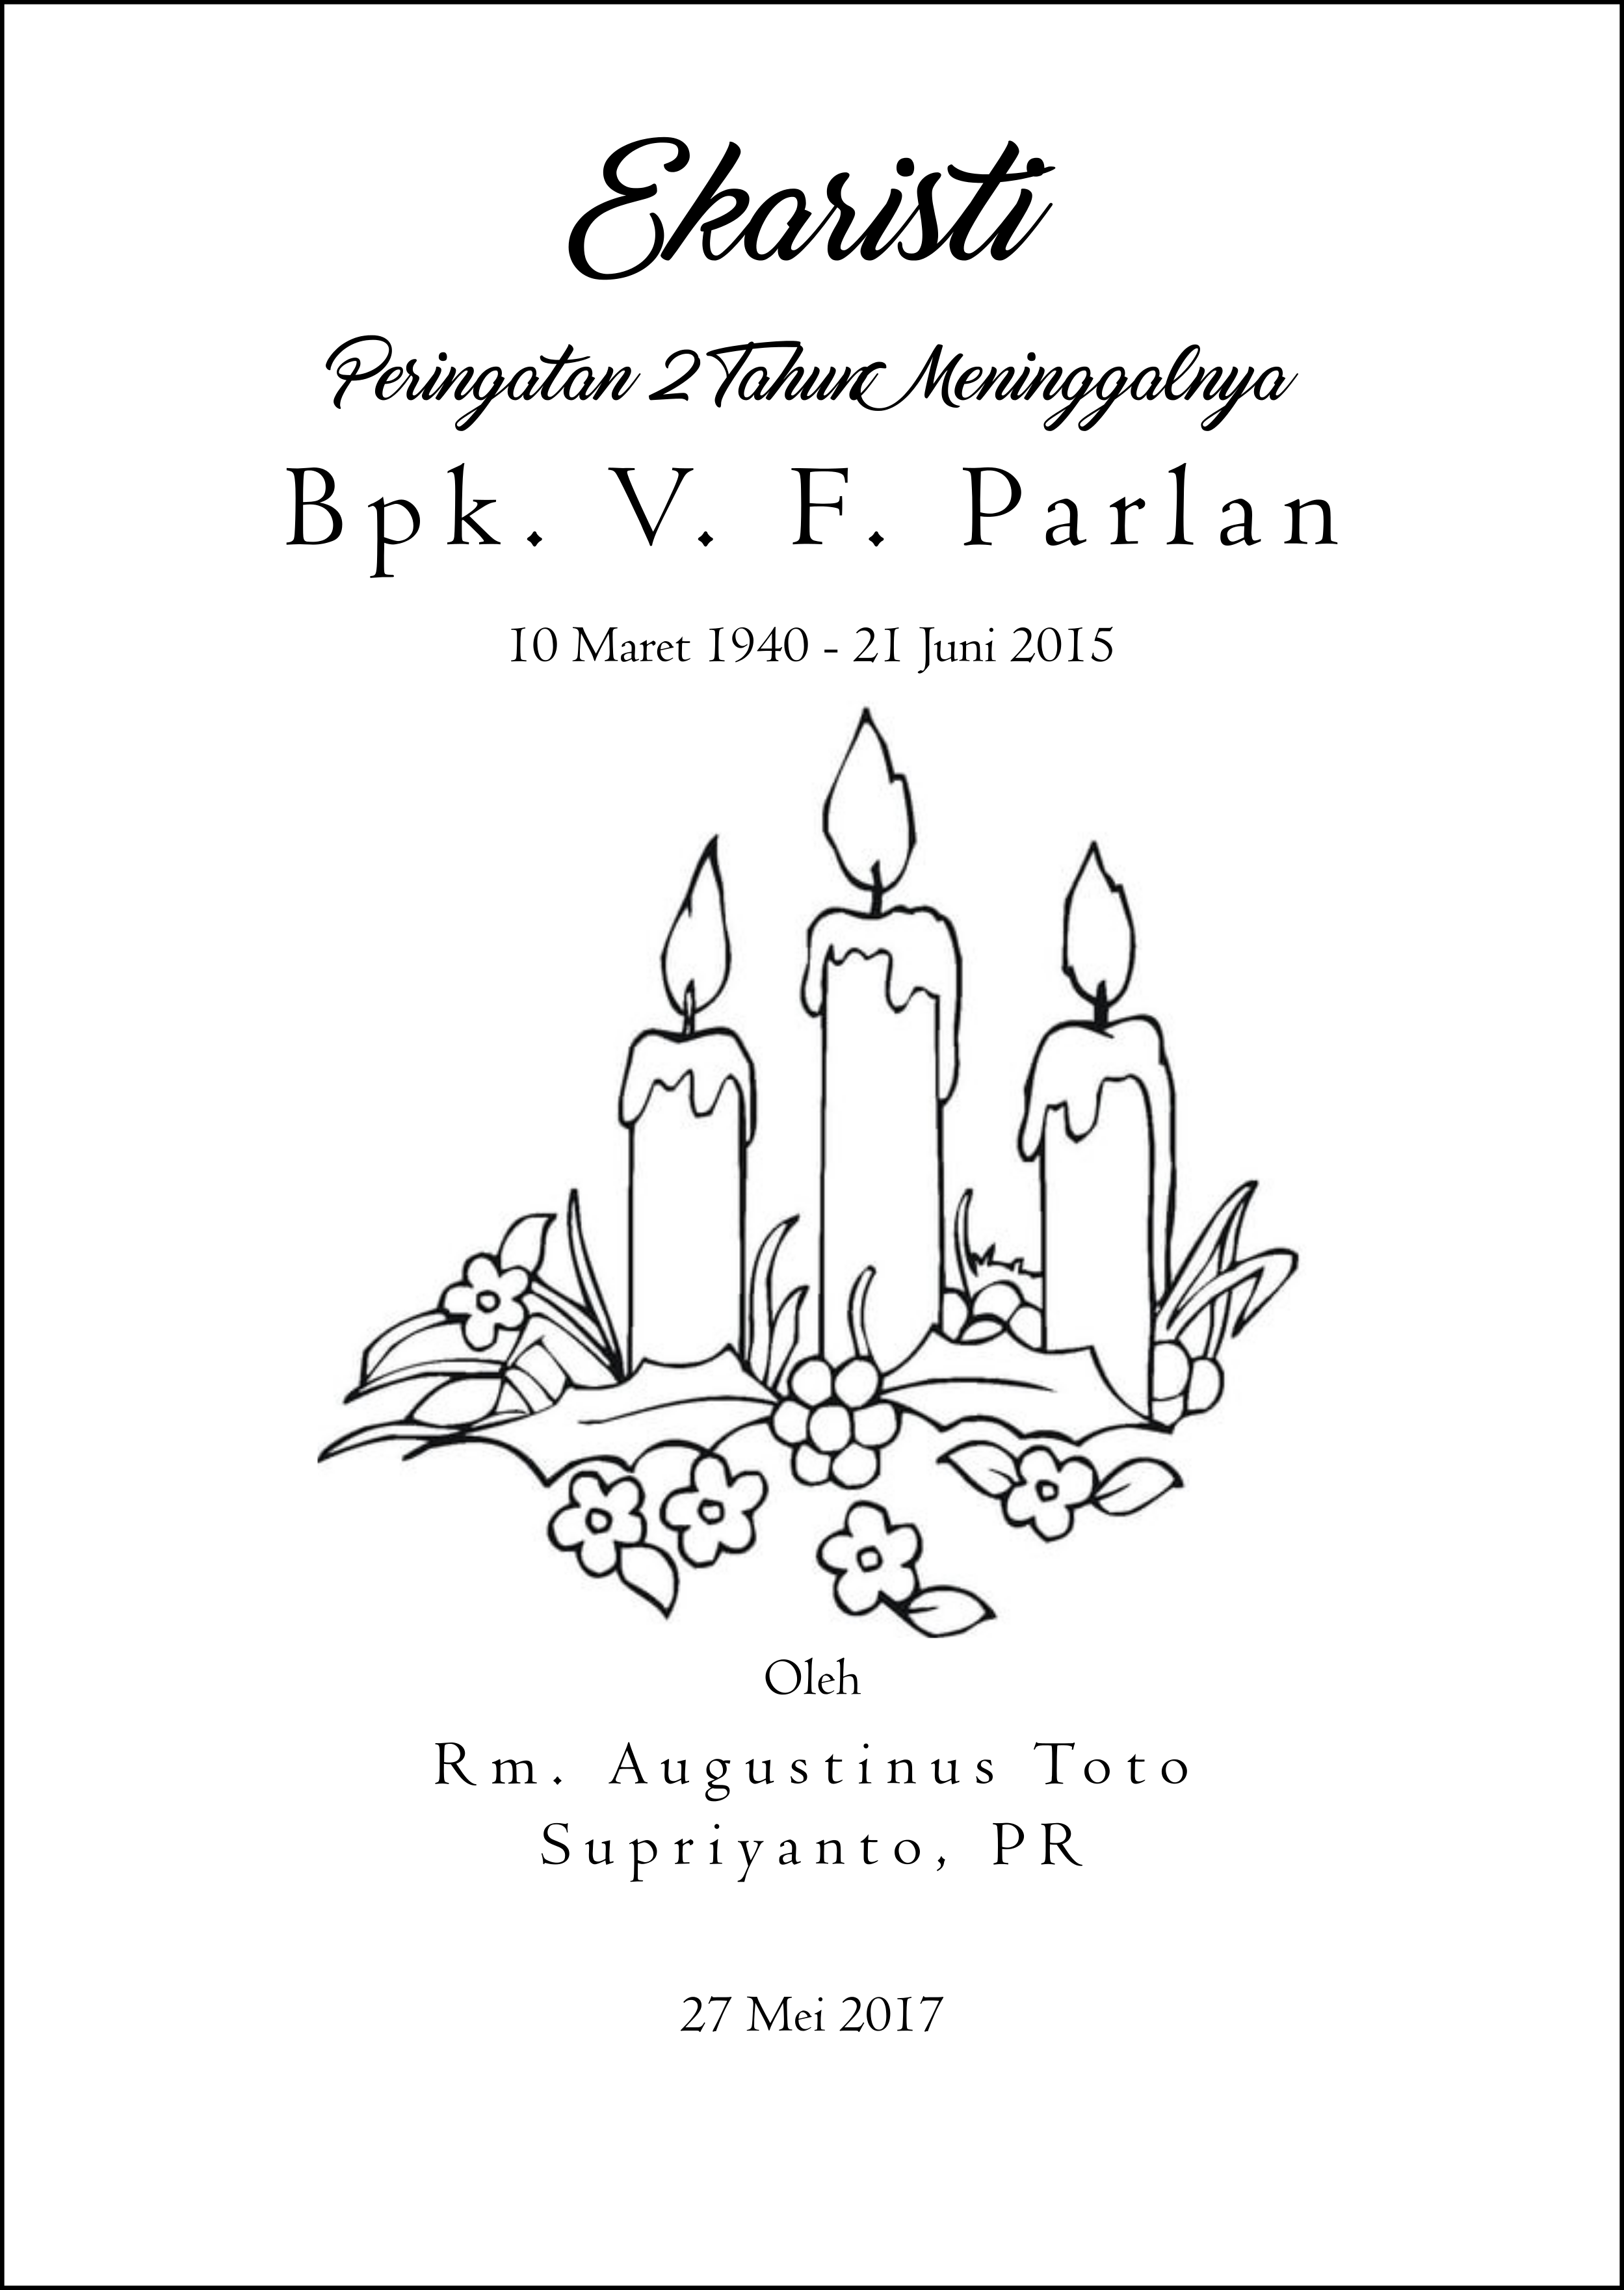
\includegraphics[scale=0.39005]{kover-ekaristi-2-tahun.png}
\end{center}

%\titleRMMH

\section*{RITUS PEMBUKA} 

 

\lagu{Lagu Pembuka}  
\small
\begin{center}
\itshape{Bila Kau Pergi}
\end{center}
\begin{verse}
	\itshape{
Bila kau pergi\\
Ke tempat yang jauh\\
Yesus s'lalu besertamu\\
Kau dibimbingNya,\\
Kau dituntunNya,\\
S'lamat seluruh langkah hidupmu\\
{~}\\
\textbf{Refr:}\\
Biar curam g'lap\\
jalan kau tempuh\\
Hatimu sedih mengerang\\
Takkan kau penat\\
Takkan kau sesat\\
bila Yesus menyertaimu\\
{~}\\
Bila kau lelah, bila kau lesu\\
Yesus slalu besertamu\\
Kau dibujukNya, kau dihiburNya\\
Slamat kau sluruh jalanmu\\
{~}\\
Biar jauh tempat yang kau tuju\\
Biar susah mencapainya\\
Kau disambutNya kau disapaNya\\
Berbahagia kau disisiNya
}
\end{verse}
\normalsize 

\subjudul{Tanda Salib} 

\BI{Demi nama  Bapa dan Putera dan Roh Kudus}

\BU{Amin}

 

\subjudul{Salam}

\BI{Semoga kasih karunia, rahmat dan damai sejahtera dari 
Allah Bapa dan dari PuteraNya Yesus Kristus beserta 
saudara.} 

\BU{Sekarang dan selama-lamanya.}

 

\subjudul{Pengantar}

\BI{Saudara-saudari yang terkasih, kita berkumpul bersama keluarga Ibu Waljiyah untuk mengenangkan belas kasih dan kemurahan hati Allah. Secara khusus kita ingin berdoa untuk saudara kita \namaalm yang telah dua tahun menghadap Allah Bapa di surga. Doa peringatan arwah seperti sekarang ini merupakan ungkapan pengharapan iman kita akan kehadiran Tahun Rahmat Tuhan, masa pembebasan bagi saudara kita itu. Pada peringatan arwah 2 tahun ini kita ingin merenungkan iman kita akan Allah Sumber Sukacita Sejati.

Semoga saudara kita \namaalm boleh menikmati sukacita sejati dan abadi di surga dan keluarga yang ditinggalkan serta kita semua juga mengalami kegembiraan sejati dalam kehidupan sehari-hari. Marilah memasuki perayaan ini dengan hati yang terbuka dan terarah kepada Allah. Kita mohon belas kasihan Allah atas segala dosa dan kelemahan kita.}


\subjudul{Tobat}

\BI{Saudara-saudara, menyadari bahwa kita hanyalah serupa 
debu bernoda di depan alas kaki Allah Bapa, marilah kita 
bersyukur bahwa kita masih diperkenankan berdoa dan 
bermohon kepada Allah Bapa. 

Saya mengaku, \ldots \ldots
} 



\BI{Semoga Allah Bapa yang Maha Kuasa, mengasihani kita, 
mengampuni dosa kita dan mengantar kita ke dalam 
kehidupan kekal.}

\BU{Amin}

\lagu{Tuhan Kasihanilah Kami} 

\subjudul{Doa Pembuka}

\BI{Marilah berdoa\\
	Allah Bapa sumber sukacita, kami telah menerima jaminan kebahagiaan abadi dalam Diri Yesus Kristus Putera-Mu. Kami serahkan hamba-Mu, \namaalm{} yang telah Engkau panggil dua tahun yang lalu dalam sukacita surgawi. Persatukanlah kami dalam pengharapan akan kebahagiaan kekal di surga, kendati masih harus berjuang di dunia ini. Bantulah kami agar memiliki sukacita sejati dan saling menghibur satu sama lain. Dengan pengantaraan Yesus Kristus PuteraMu Tuhan kami yang bersama dengan Dikau dalam persekutuan Roh Kudus hidup dan berkuasa, Allah sepanjang segala masa.}

\BU{Amin}

 

\section*{LITURGI SABDA} 

\keterangan{Pembacaan dari Surat Paulus kepada umat di
Korintus (2 Kor 1:3-7)}

\BP{Terpujilah Allah, Bapa Tuhan kita Yesus Kristus, Bapa yang penuh belas
	kasih dan Allah sumber segala penghiburan. Ia menghibur kami dalam
	segala penderitaan, sehingga kami sanggup menghibur semua orang
	yang berada dalam macam-macam penderitaan dengan penghiburan
	yang kami terima sendiri dan Allah. Sebab seperti halnya kami
	mendapat bagian berlimpah dalam kesengsaraan Kristus, demikian pula
	berlimpahlah penghiburan kami oleh Kristus. Jika kami menderita, hal
	itu menjadi penghiburan dan keselamatan kamu; jika kami dihibur,
	maka hal itu adalah untuk penghiburan kamu, sehingga kamu beroleh
	kekuatan untuk dengan sabar menderita kesengsaraan yang sama
	seperti yang kami derita juga. Dan pengharapan kami akan kamu adalah
	teguh, karena kami tahu, bahwa sama seperti kamu turut mengambil
	bagian dalam kesengsaraan kami, kamu juga turut mengambil bagian
	dalam penghiburan kami. 
	
	
Demikianlah Sabda Tuhan.}

\BU{Syukur kepada Allah}

\lagu{Lagu tanggapan sabda}
\small
\begin{center}
\itshape{Ku mohon ya Tuhan - MB 218}
\end{center}
\begin{verse}
\itshape{
Ku mohon ya Tuhan, 
buka hati hamba\\
Buatlah hamba 
mampu mendengar sabdaMU\\
{~}\\
Gemakan ya Tuhan, 
lagu panggilanMU\\
Supaya jiwaku 
mengidungkan perintahMu\\
{~}\\
Tiuplah nada, 
sabda sangkakala\\
Supaya umatMu
melaksanakan sabdaMu}
\end{verse}
\normalsize


 

\subjudul{Injil}

\BI{Tuhan sertamu}

\BU{dan sertamu juga} 

\BI{Inilah Injil Yesus Kristus menurut Yohanes (15:9-12)}

\BU{Dimuliakanlah Tuhan}

\BI{\textit{Tinggallah di dalam kasih-Ku, supaya sukacitamu menjadi penuh.}
	
	Dalam amanat perpisahan-Nya Yesus berkata kepada murid-murid-Nya,
	"Seperti Bapa telah mengasihi Aku, demikianlah juga Aku telah
	mengasihi kamu; tinggallah di dalam kasih-Ku itu. Jikalau kamu
	menuruti perintahKu kamu akan tinggal di dalam kasih-Ku, seperti Aku
	rnenuruti perintah Bapa-Ku dan tinggal di dalarn kasih-Nya.
	Semuanya itu Kukatakan kepadamu supaya sukacita-Ku ada di dalam
	kamu dan sukacitamu menjadi penuh. Inilah perintah-Ku yaitu supaya
	kamu saling mengasihi, seperti Aku telah mengasihi kamu."
}


\BI{Demikianlah Injil Tuhan}

\BU{Terpujilah Kristus}

 

\subjudul{Homili}

\subjudul{Syahadat} 

\subjudul{Doa Umat}

\BI{Saudara-saudari, kehadiran kita bersama di sini adalah untuk mengungkapkan iman kita akan Allah sumber sukacita sejati. Marilah dengan rendah hati kita ungkapkan doa dan permohonan kita kepada Bapa:}
% % %
\BP{Ya Bapa, kedatangan Yesus Kristus di tengah-tengah kami menghadirkan tahun rahmat Tuhan kepada umat manusia. Semoga, peringatan dua tahun meninggalnya saudara kami \namaalm ini pun, menghadirkan rahmat bagi saudara-saudari yang ditinggalkan dan kami semua yang hadir di sini.

\textit{Hening sejenak \ldots\ldots} 

Marilah kita mohon :}

\BU{Kabulkanlah doa kami ya Tuhan}


\BP{Ajarkanlah kepada kami iman, harapan, dan kasih yang sejati, agar kami mampu mengalami sukacita sejati baik di dunia ini maupun dalam persekutuan para kudus sebagaimana telah dialami oleh saudara kami \namaalm ini. 

\textit{Hening sejenak \ldots\ldots} 

Marilah kita mohon :}

\BU{Kabulkanlah doa kami ya Tuhan.}

\BP{Bantulah kami untuk meyakini bahwa hidup bukanlah berakhir di dunia ini, namun tetap berlanjut dalam kehidupan abadi bersamaMu. Semoga dalam peziarahan yang penuh tantangan ini kami tetap mampu memancarkan kegembiraan dan sukacita sejati. 

\textit{Hening sejenak \ldots\ldots} 

Marilah kita mohon :}

\BU{Kabulkanlah doa kami ya Tuhan.}

\BP{Ya Bapa, bantulah kami yang masih berjuang ini untuk meneruskan teladan dan ajaran kasih Putra-Mu, Yesus Kristus di tengah-tengah dunia yang penuh tantangan ini.

\textit{Hening sejenak \ldots\ldots} 

Marilah kita mohon :}

\BU{Kabulkanlah doa kami ya Tuhan.}

\BP{Bagi semua orang yang meninggal terutama Bapak dan Ibu Karsodinomo, Bapak dan Ibu Parjosuwito, Bapak dan Ibu Siswosudarmo, Bapak Ignatius Subiyatmo, Bapak Petrus Slamet Handoko dan Ibu Monica Soehartati, serta Bapak Atun Hudori, semoga karena kerahiman Tuhan mereka diijinkan memandang
	kemuliaan wajah Allah.
	
	\textit{Hening sejenak \ldots\ldots} 
	
	Marilah kita mohon :}

\BU{Kabulkanlah doa kami ya Tuhan.}

\BI{Bapa, kasih-Mu tiada batas. Kesabaran-Mu begitu besar. Semoga dalam pengharapan iman yang benar, kami mampu mewujudkan permohonan kami ini dalam limpahan rahmat-Mu. Dengan pengantaraan Kristus, Tuhan kami.}

\BU{Amin}

\section*{LITURGI EKARISTI}

\lagu{Lagu pengantar persembahan}
\small
\begin{center}
	\itshape{Trimalah Persembahan Kami}
\end{center}
\begin{verse}
	\itshape{
Kau perkenankan kami hadir\\
di dalam pesta ini\\
Meskipun kami tak layak mendapatkan\\
 belas kasihanMu.\\
{~}\\
Semoga berkat kurban ini\\
 Kau menyucikan kami\\
Sehingga layak dan pantas\\
menghantarkan persembahan ini\\
{~}\\
Trimalah persembahan kami:\\ 
roti dan anggur ini,\\
bersama dengan semua yang kami miliki.\\ 
Semoga Kau berkenan.\\ 
{~}\\
Semoga Tubuh dan DarahMu\\ 
yang akan kami sambut,\\ 
membawa kami menuju kehidupan kekal\\ 
bersamaMu di surga. 
}
\end{verse}
\normalsize

\BI{Kami memuji Engkau ya Bapa, Allah semesta alam, sebab 
dari kemurahanMu kami menerima roti dan anggur yang 
kami persembahkan ini. Inilah hasil dari bumi dan usaha 
manusia yang bagi kami akan menjadi santapan rohani.}

\BU{Terpujilah Allah selama-lamanya}

\BI{Berdoalah saudara-saudara supaya persembahan kita ini 
diterima oleh Allah Bapa yang mahakuasa.}

\BU{Semoga persembahan ini diterima demi kemuliaan Tuhan 
dan keselamatan kita serta seluruh umat Allah yang kudus.}

\BI{Allah Bapa sumber kekudusan, terimalah bahan persembahan roti dananggur yang kami unjukkan untuk keselamatan hamba-Mu \namaalm. Bersama dengan keteguhan hati kami yang percaya akanbelas kasihan-Mu. Kami percayakan arwah sanak-saudara kami yang telah  berpulang,  juga   hamba-Mu  \namaalm,  yang  telahseribu   hari   menghadap-Mu   ke   dalam     pangkuan   kasih-Mu   di   surga. Dengan pengantaraan Kristus, Tuhan kami.}

\BU{Amin} 

\subjudul{DOA SYUKUR AGUNG}


\subjudul{Kudus}

\subjudul{Bapa Kami}

\subjudul{Anak Domba Allah}

\subjudul{Komuni}
\newpage
\subjudul{Lagu Komuni}
\small
\begin{center}
	\itshape{Indah RencanaMu}
\end{center}
\begin{verse}
	\itshape{
Indah rencanaMu Tuhan,\\ 
di dalam hidupku\\
Walau 'ku tak tahu\\ 
dan 'ku tak mengerti\\ 
semua jalanMu\\
{~}\\
Dulu 'ku tak tahu Tuhan,\\ 
berat kurasakan\\
Hati menderita\\ 
dan 'ku 'tak berdaya\\ 
menghadapi semua\\
{~}\\
Tapi 'ku mengerti s'karang, Kau tolong padaku\\
Kini 'ku melihat dan 'ku merasakan indah recanaMu\\
Kini 'ku melihat dan 'ku merasakan indah recanaMu\\
}
\end{verse}
\normalsize 

\subjudul{Doa sesudah komuni}

\BI{Marilah berdoa: 
	
	Allah Bapa yang Mahabaik, kami telah menyambut rejeki surgawi pada peringatan   seribu   hari   hamba-Mu  \namaalm   berada  dalamrumah-Mu yang abadi.  Semoga berkat Ekaristi Suci ini kami bertekun dalam iman, harapan, dan kasih, dan saudara kami \namaalm itu   menjadi   pendoa   bagi   kami   yang   masih   melanjutkan   pengabdian kami. Semoga  kami  siap  siaga  selalu  menyambut kehadiranMu  yang menyelamatkan. Dengan pengantaraan Kristus, Tuhan kami.}

\BU{Amin.}

 

\section*{RITUS PENUTUP}

\BI{Tuhan beserta kita}

\BU{Sekarang dan selama-lamanya}

\BI{Semoga saudara sekalian diberkati oleh Allah Yang 
Mahakuasa \Cross ~Bapa dan Putera dan Roh Kudus.}

\BU{Amin}

 

\subjudul{Pengutusan}

\BI{Saudara sekalian, Perayaan Ekaristi untuk memohon 
berkat Allah Bapa bagi arwah \namaalm telah selesai.}

\BU{Syukur kepada Allah}

\BI{Kita diutus untuk mewartakan bahwa Tuhan Yesus adalah 
jalan, kebangkitan dan hidup.}

\BU{Amin.}

 

\lagu{Lagu Penutup}

\scriptsize
\begin{center}
	\itshape{nDh\`{e}r\`{e}k Gusti}
\end{center}
\begin{verse}
	\itshape{
Y\'{e}n atimu krasa ora tentrem, \\
awan bengi ora bisa merem\\
Aja nganti kow\'{e} njur salah dalan,\\
bingung pikiran lunga saparan-paran.\\
{~}\\
Rajabrana ra marakk\'{e} ayem,\\ 
pangkat mulya ra ndad\`{e}kk\'{e} tentrem\\
Ng\`{e}lingana donyan\'{e} kebak godha,\\ 
sapa l\'{e}na urip\'{e} bakal cilaka.\\
{~}\\
\textbf{Ref:}\\
Ndh\`{e}r\`{e}k Gusti Y\'{e}sus ati ayem, \\
dalan padhang pikiran dadi tenang\\
Ndh\`{e}r\`{e}k Gusti Y\'{e}sus ati tentrem, \\
sapa wong\'{e} sing ngandel lan pracaya\\
{~}\\
Ndh\`{e}r\`{e}k Gusti, atimu sing suci,\\
ndh\`{e}r\`{e}k Gusti, pasrah lan ngabekti\\
Ng\`{e}lingana Gusti nat\'{e} ngandika, \\
sing pracaya bakal\'{e} mlebu swarga
		
}
\end{verse}
\normalsize 

\newpage
\begin{flushright}
{\Large Ucapan terima kasih}\\
\noindent Dengan penuh syukur dalam kasih Tuhan, kami mengucapkan banyak
terima kasih kepada:
\large

\textbf{Romo \namaromo}\\
yang telah berkenan memimpin perayaan ekaristi peringatan 2 tahun meninggalnya\\ \namaalm
ini.

\textbf{Koor Calista}\\
yang telah menyemarakkan perayaan ekaristi ini.

\textbf{Umat lingkungan St. Yustinus, para undangan, segenap keluarga, dan orang-orang terkasih}\\
yang telah berkenan hadir memberikan cinta dan doa dalam perayaan
ekaristi ini.

Semoga Tuhan memberkati dan memelihara ikatan kasih\\ di antara kita semua.

Amin.

\bigskip 

\textit{Ibu MG Waldjijah\\
dan segenap keluarga}
\end{flushright}

\end{document} 

[07:09, 5/24/2016] +62 813-2829-0020: 
Pembk hatiku percaya, antar bacaan keheningan hati, persembahan terimalah syukur kami, Kom bagaikan rusa rindukan sungaimu, penutup Asmo Dalem Maria.
[07:09, 5/24/2016] +62 813-2829-0020: Lagu misa tgl 4 Juni, ordinarium Lauda sion

Undefined control sequence. Marilah kita mohon :}